\documentclass{scrartcl}
\usepackage{amsmath,amssymb,commath,graphicx,enumerate,listings}
\setkomafont{disposition}{\normalfont\bfseries}

\title{Mat 354}
\subtitle{Homework 6}
\author{Kenny Roffo}
\date{Due October 12, 2015}

\begin{document}
\maketitle

All calculations were done in R.

\begin{enumerate}

\item Let the random variable $Y$ have the probability function $$p(y) = \frac{(|y|+1)^2}{18}\text{\hspace{.5in}}y=-2,-1,0,1$$ Determine values for

\begin{enumerate}[a)]
\item $E(Y)$:\\

\begin{align*}
  E(Y) &= \sum_{y=-2}^1\left(yp(y)\right)\\
       &= -1
\end{align*}

\item $E(Y^2)$:\\
\begin{align*}
  E(Y^2) &= \sum_{y=-2}^1\left(y^2p(y)\right)\\
       &= 2.4444
\end{align*}

\item $V(Y)$:\\
\begin{align*}
  V(Y) &= E(Y^2) - E(Y)\\
       &= 2.4444 - (-1)\\
       &= 3.4444
\end{align*}

\item The standard deviation of $Y$:\\
  \begin{align*}
    \sigma &= \sqrt{V(Y)}\\
           &= \sqrt{3.4444}\\
           &= 1.8559
  \end{align*}

\item $E(3Y^2-2Y+4)$:\\
\begin{align*}
  E(Y^2) &= \sum_{y=-2}^1\left((3y^2-2y+4)p(y)\right)\\
       &= 13.3333
\end{align*}
\end{enumerate}

\item Monthly unit sales $Y$ of a product vary. The expected monthly sales is 1200 units; the standard deviation of the monthly sales is 120 units. It costs \$6200 per month to maintain the sales staff, \$11 per item to manufacture, and each item is sold for \$18.

\begin{enumerate}[a)]
\item If profit is denoted $X$, write $X$ as a function of unit sales $Y$.\\
$$X(Y) = (18 - 11)Y - 6200 = 7Y - 6200$$

\item Determine the expected value of the monthly profit.\\
\begin{align*}
  E(X) &= X(E(Y))\\
       &= X(1200)\\
       &= 7(1200) - 6200\\
       &= 7200
\end{align*}

Thus the expected monthly profit is \$7200

\item Determine the variance of the monthly profit.\\
\begin{align*}
  V(X) &= 7^2V(Y)\\
       &= 49(120)\\
       &= 5880
\end{align*}

\item Determine the standard deviation of the monthly profit.\\
\begin{align*}
  SD(X) &= |7|SD(Y)\\
       &= 7\sqrt{120}\\
       &= 76.68
\end{align*}
\end{enumerate}

\item Consider the situation posed in Exercise 3.44b $(p=.6)$, but with a change of sample size from 5 to $n$. If $Y$ is the number of successful surgeries, then sample proportion of successes is $Y/n$. Find the probability that this sample proportion falls between 0.55 and 0.651 for samples of size:

\begin{enumerate}[a)]
\item 24:\\
\begin{align*}
  P(0.55\le Y/n\le0.651) &= P(0.55n\le Y \le0.651n)\\
  &= P(13.2\le Y\le 15.624)\\
  &= P(13\le Y \le15)\\
  &= P(Y\le15) - P(Y\le13)\\
  &= 0.3223 \text{\hspace{0.5in} Using pbinom in R}
\end{align*}

\item 96:\\
\begin{align*}
  P(0.55\le Y/n\le0.651) &= P(0.55n\le Y \le0.651n)\\
  &= P(52.8\le Y\le 62.496)\\
  &= P(53\le Y \le62)\\
  &= P(Y\le62) - P(Y\le53)\\
  &= 0.6503
\end{align*}


\item 384:\\
\begin{align*}
  P(0.55\le Y/n\le0.651) &= P(0.55n\le Y \le0.651n)\\
  &= P(211.75\le Y\le 250.635)\\
  &= P(212\le Y \le250)\\
  &= P(Y\le250) - P(Y\le212)\\
  &= 0.9517
\end{align*}


\item What happens to this probability as the sample size is increased?\\

  It increases.

\end{enumerate}\pagebreak

\item Singulair is a medication used to control asthma. In clinical trials of Singulair, 18.4\% of patients in a large study experienced headaches as a side effect. Take it for granted, then, that when a new patient is prescribed Singulair, the probability is $p = 0.816$ that they do not experience a headache.

\begin{enumerate}[a)]
\item Who manufactures Singulair?\\
Merck \& Co.

\item All drugs eventually go off patent, at which time the company that developed the drug loses a major source of revenue / profit. It’s in the company’s best interest to develop derivative drugs that at least incrementally improve upon the original, get this “new” drug patented, and continue to profit (without expending as many resources as is required to develop a novel compound from scratch).

The Singulair people have such an inexpensive derivative in mind – Dyadair – and their hope is that the justification for this new drug will involve an improvement in the side effect profile. 50 randomly selected asthma sufferers are enrolled into a trial. Take Y to be the number who experience side effects.

In solving what follows, take the point of view that Singulair derivatives (Dyadair is one) that are under consideration are identical to the original Singulair with respect to side effects.

That is: $p = 0.816$.\\

For our first derivative Dyadair.\\

Construct and print a plot, in R, of the probability function for $Y$.\\
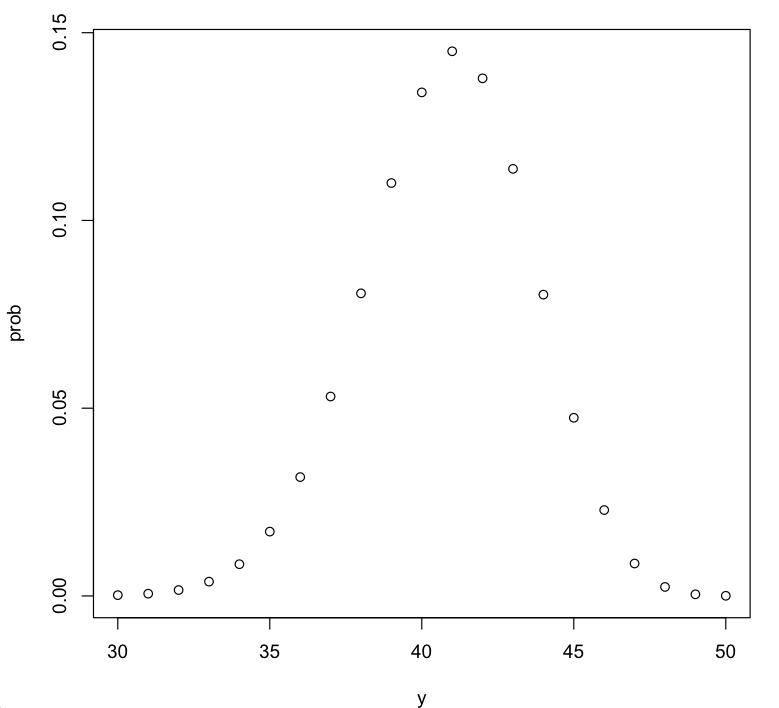
\includegraphics[keepaspectratio=true, scale=0.5]{4b.png}\\

\item Determine the expected value, variance, and standard deviation of the distribution.\\

Since this is a binomial setting, I am using the formulas for a binomial distribution:
\begin{align*}
  E(Y) &= np\\
       &= (50)(0.816)\\
       &= 40.8\\
  V(Y) &= np(1-p)\\
       &= (50)(0.816)(0.184)\\
       &= 7.5072\\
  SD(Y) &= \sqrt{V(Y)}\\
        &= \sqrt{7.5072}\\
        &= 2.7399
\end{align*}

\item The company's statisticians set the following criterion: If the number of people who do not have a side effect is at least 46 (that is: 92\% of the sample – well above 81.6\%), we will continue to develop Dydair. If not, we'll stop. For the case where $p = 0.816$, what is $P(Y \ge 46)$? Do you see why this rule would be effective in preventing the company from acting in a situation where the true state of things is one of no change?\\
\begin{align*}
  P(Y\ge46) &= 1 - P(Y\le45)\\
            &= 1 - 0.9656 \text{\hspace{0.5in}Calculated with pbinom}\\
            &= 0.0344
\end{align*}
Yes I see why that is an effective rule.

\end{enumerate}

\item (The problem of multiple comparisons) Continuation of 4. These go back to issues we’ve been working on all semester. You can’t tackle them until you’re solid on \#4.

Now – it turns out that pharmaceutical companies have lots of ways to slightly alter a drug. Suppose 40 such alterations are in store for Singulair – all with identical side effect profile to that of Singulair. (In short: No improvements at all.) For each of these 40 derivative drugs a study involving 50 asthmatics is conducted. Assume all 40 studies are independent (they do not share the same subjects).

\begin{enumerate}[a)]
\item Obtain the probability that the maximum count (the maximum $Y$), over the 40 different studies, is at least 46.\\

\begin{align*}
  P(Y\ge46) &= 1 - 0.9656^{40} \text{\hspace{0.5in}(from the calculation of 4d)}\\
            &= 0.7535
\end{align*}

\item Take $p_{Max}$ to be the probability function for the maximum value obtained in the 40 studies. Produce a plot of this function (restrict the plot to values from 40 to 50).\\
Here is the code I used to get this plot:
\begin{lstlisting}[language=R]
  y <- seq(0,50)
  maxProbs <- pbinom(y,50,0.816)^40
            - pbinom(y-1,50,0.816)^40
  plot(y, maxProbs, xlim = c(40,50), type="h")
\end{lstlisting}

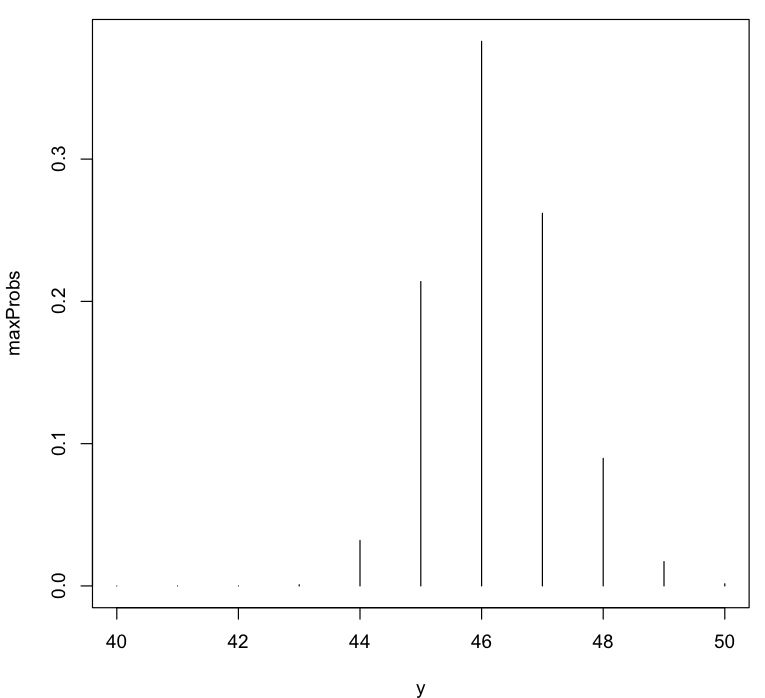
\includegraphics[keepaspectratio=true, scale=0.5]{5b.png}\\


\item (Look at your plot.) I am almost certain that the maximum will be at least \underline{43}.\pagebreak

\item Determine the expected value, variance and standard deviation of the maximum.\\
  \begin{lstlisting}[language=R]
  sum(maxProbs*y)
  \end{lstlisting}
  gives $E(Y) = 46.2183$

  \begin{lstlisting}[language=R]
  sum(maxProbs*y^2) - sum(maxProbs*y)^2
  \end{lstlisting}
  gives $V(Y) = 1.1018$

  And $SD(Y) = 1.0947$
\end{enumerate}
\end{enumerate}
\end{document}

